\documentclass[12pt, twoside]{article}
\usepackage[letterpaper, margin=1in, headsep=0.5in]{geometry}
\usepackage[english]{babel}
\usepackage[utf8]{inputenc}
\usepackage{amsmath}
\usepackage{amsfonts}
\usepackage{amssymb}
\usepackage{tikz}
%\usetikzlibrary{quotes, angles}

\usepackage{graphicx}
\usepackage{enumitem}
\usepackage{multicol}

\usepackage{fancyhdr}
\pagestyle{fancy}
\fancyhf{}
\renewcommand{\headrulewidth}{0pt} % disable the underline of the header

\fancyhead[RE]{\thepage}
\fancyhead[RO]{\thepage \\ Name: \hspace{3cm}}
\fancyhead[L]{BECA / Dr. Huson / 10th Grade Geometry\\* 4 January 2019}

\begin{document}
\subsubsection*{Do Now: Solving situations using algebra}
 \begin{enumerate}

 \item $\triangle ABC$ is shown with $m\angle C=90^\circ$. Given $m\angle A =30^\circ$, and the lengths of the triangle's sides are $a$, $b$, and $c=10$. \vspace{0.1cm}
   \begin{multicols}{2}
       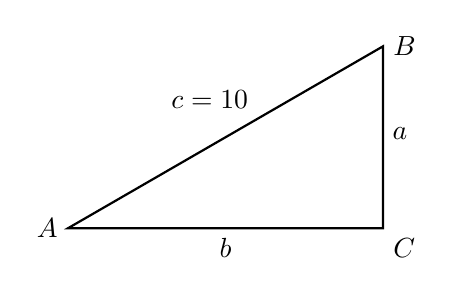
\begin{tikzpicture}%[scale=0.7]
         \draw [thick]
         (0,0)node[left]{$A$}--
         (4,0)node[below right]{$C$}--
         (4,2.31)node[right]{$B$}--cycle;
         \node at (2,0)[below]{$b$};
         \node at (4,1.2)[right]{$a$};
         \node at (1.8,1.4)[above]{$c=10$};
       \end{tikzpicture}

       \begin{enumerate}
       \item Solve for $a$ using $\displaystyle \sin 30^\circ =\frac{a}{10}$ \vspace{0.75cm}
       %\item $\cos A =$ \vspace{0.75cm}
       %\item $\tan A =$
     \end{enumerate}
   \end{multicols} \vspace{1cm}

 \item Solve for the length, $c$, of the hyptenuse of a right triangle where one angle has measure $35^\circ$ and the length of the side opposite it is 11.4. That is, solve for $c$: $\displaystyle \sin 35^\circ =\frac{11.4}{c}$.  \vspace{4cm}

 \item Find the area of $\triangle ABC$,  $Area= \frac{1}{2}bh$. The altitude $h$ of the triangle is 75 centimeters and the base $AB=110$ cm.\\[0.5cm]
 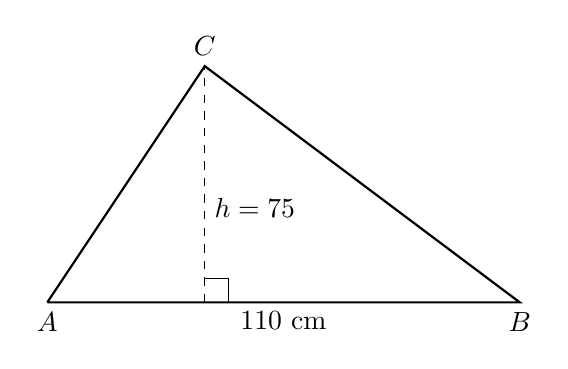
\begin{tikzpicture}%[scale=0.7]
   \draw [thick]
     (2,0)node[below]{$A$}--
     (8,0)node[below]{$B$}--
     (4,3)node[above]{$C$} --(2,0);
  \draw [dashed] (4,0)--(4,3);
  \draw (4,0)++(0.3,0)--++(0,0.3)--+(-0.3,0);
  \node at (4,1.2)[right]{$h=75$};
  \node at (5,0)[below]{$110$ cm};
\end{tikzpicture} \vspace{0.5cm}

\item The area of a triangular banner is 12710 square centimeters. If the base is 155 cm long, what is the banner's height?

\end{enumerate}
\end{document}
